\begin{frame}{Whats wrong?}

  \begin{figure}
    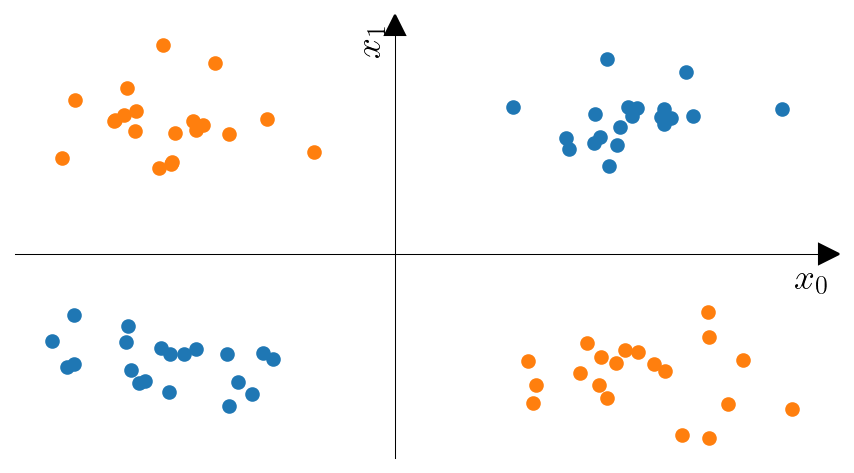
\includegraphics[width=0.45\textwidth]{classification_xor}
    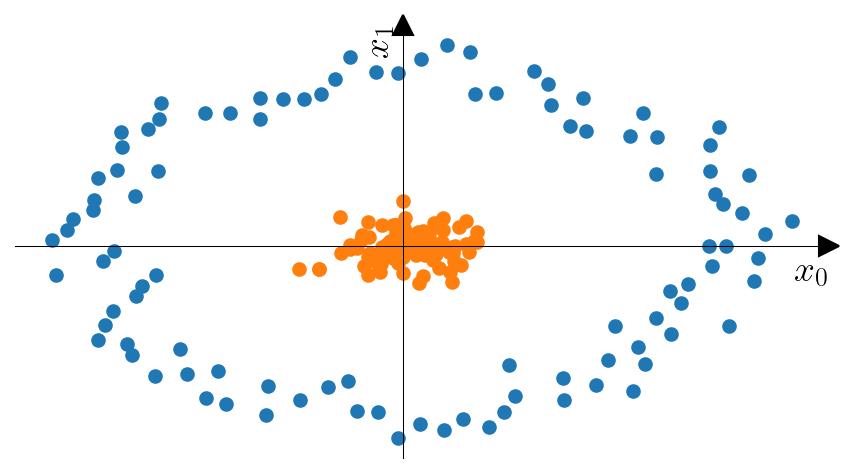
\includegraphics[width=0.45\textwidth]{classification_sin}
  \end{figure}

  \note{
    \begin{itemize}
      \item Not all data distributions can be classified like this.
    \end{itemize}
  }
\end{frame}



\begin{frame}{So far we solved this with feature engineering.}
  \begin{figure}
    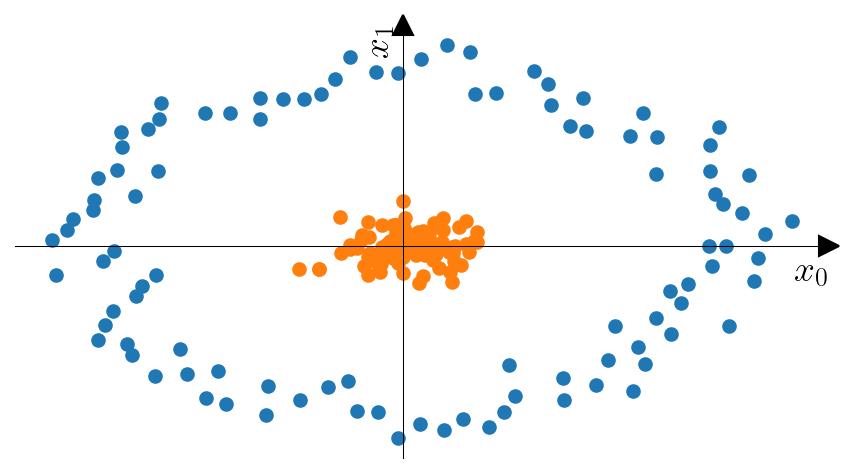
\includegraphics[width=0.45\textwidth]{classification_sin}
    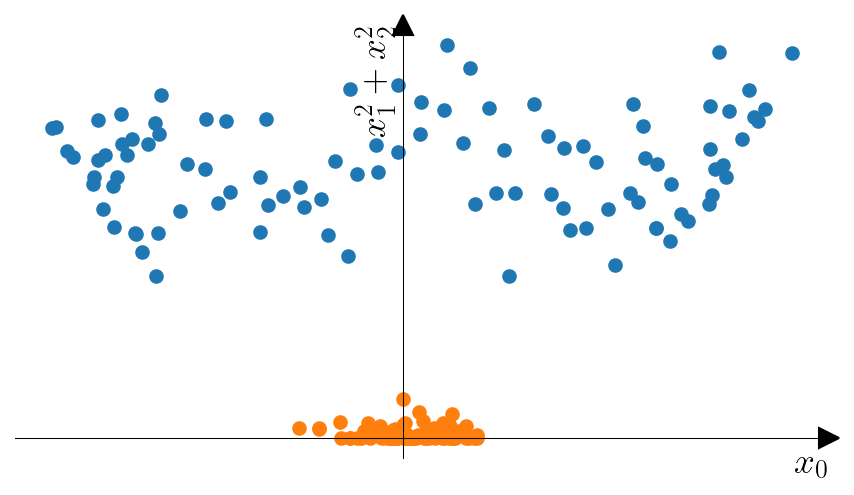
\includegraphics[width=0.45\textwidth]{classification_sin_mapped}
  \end{figure}

  \note{
    \begin{itemize}
      \item We mapped the images from the highly complex pixel space using e.g. SIFT or HOG into a feature space.
      \item And afterwards hoped for a good classification result in feature space using e.g. SVM.
    \end{itemize}
  }
\end{frame}


\begin{frame}{Can we learn these mappings?}

  \begin{columns}
    \begin{column}{0.48\textwidth}
      \begin{figure}
        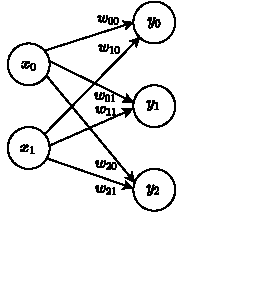
\includegraphics[width=0.9\textwidth]{neuron_00}
      \end{figure}
    \end{column}
    \begin{column}{0.48\textwidth}
      \begin{align*}
        y &= \sigma(Wx) \\
      \end{align*}
    \end{column}
  \end{columns}

  \note{
    \begin{itemize}
      \item Our starting point the linear classifier.
      \item Let's add another mapping into our Logistic Regression!
    \end{itemize}
  }
\end{frame}


\begin{frame}{Can we learn these mappings?}

  \begin{columns}
    \begin{column}{0.48\textwidth}
      \begin{figure}
        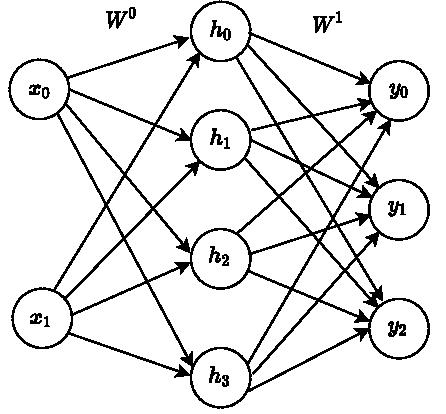
\includegraphics[width=0.9\textwidth]{neuron_01}
      \end{figure}
    \end{column}
    \begin{column}{0.48\textwidth}
      \begin{align*}
        y &= \sigma(W^{1}\phi(W^{0}x)) \\
        h &= \phi(W^{0}x)
      \end{align*}
    \end{column}
  \end{columns}

  \note{
    \begin{itemize}
      \item The vector $h$ is a representation in a learned feature space. \\
      $\rightarrow$ It can have any dimensionality.
      \item $\phi$ is called the activation function. \\
      $\rightarrow$ It needs to be non-linear. A purely linear mapping into a new feature space wouldn't help.
    \end{itemize}
  }
\end{frame}


\begin{frame}{Can we learn these mappings? $\rightarrow$ Artificial Neural Network}
  \begin{figure}
    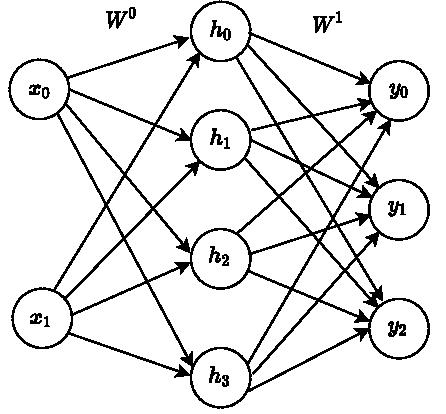
\includegraphics[width=0.6\textwidth]{neuron_01}
  \end{figure}
  \note{
    \begin{itemize}
      \item This is what is called an Artificial Neural Network with one hidden layer.
      \item It's also sometimes called a Multilayer Perceptron (MLP).
      \item Universal Approximation Theorem: \\
            A neural network with one hidden layer can learn to approximate any continuous function. The quality of the approximation depends on the number of hidden neurons (size of the hidden layer).\\
            \url{https://en.wikipedia.org/wiki/Universal_approximation_theorem}
    \end{itemize}
  }
\end{frame}


\begin{frame}{Can we learn these mappings? $\rightarrow$ Artificial Neural Network}

  \begin{columns}
    \begin{column}{0.48\textwidth}
      \begin{figure}
        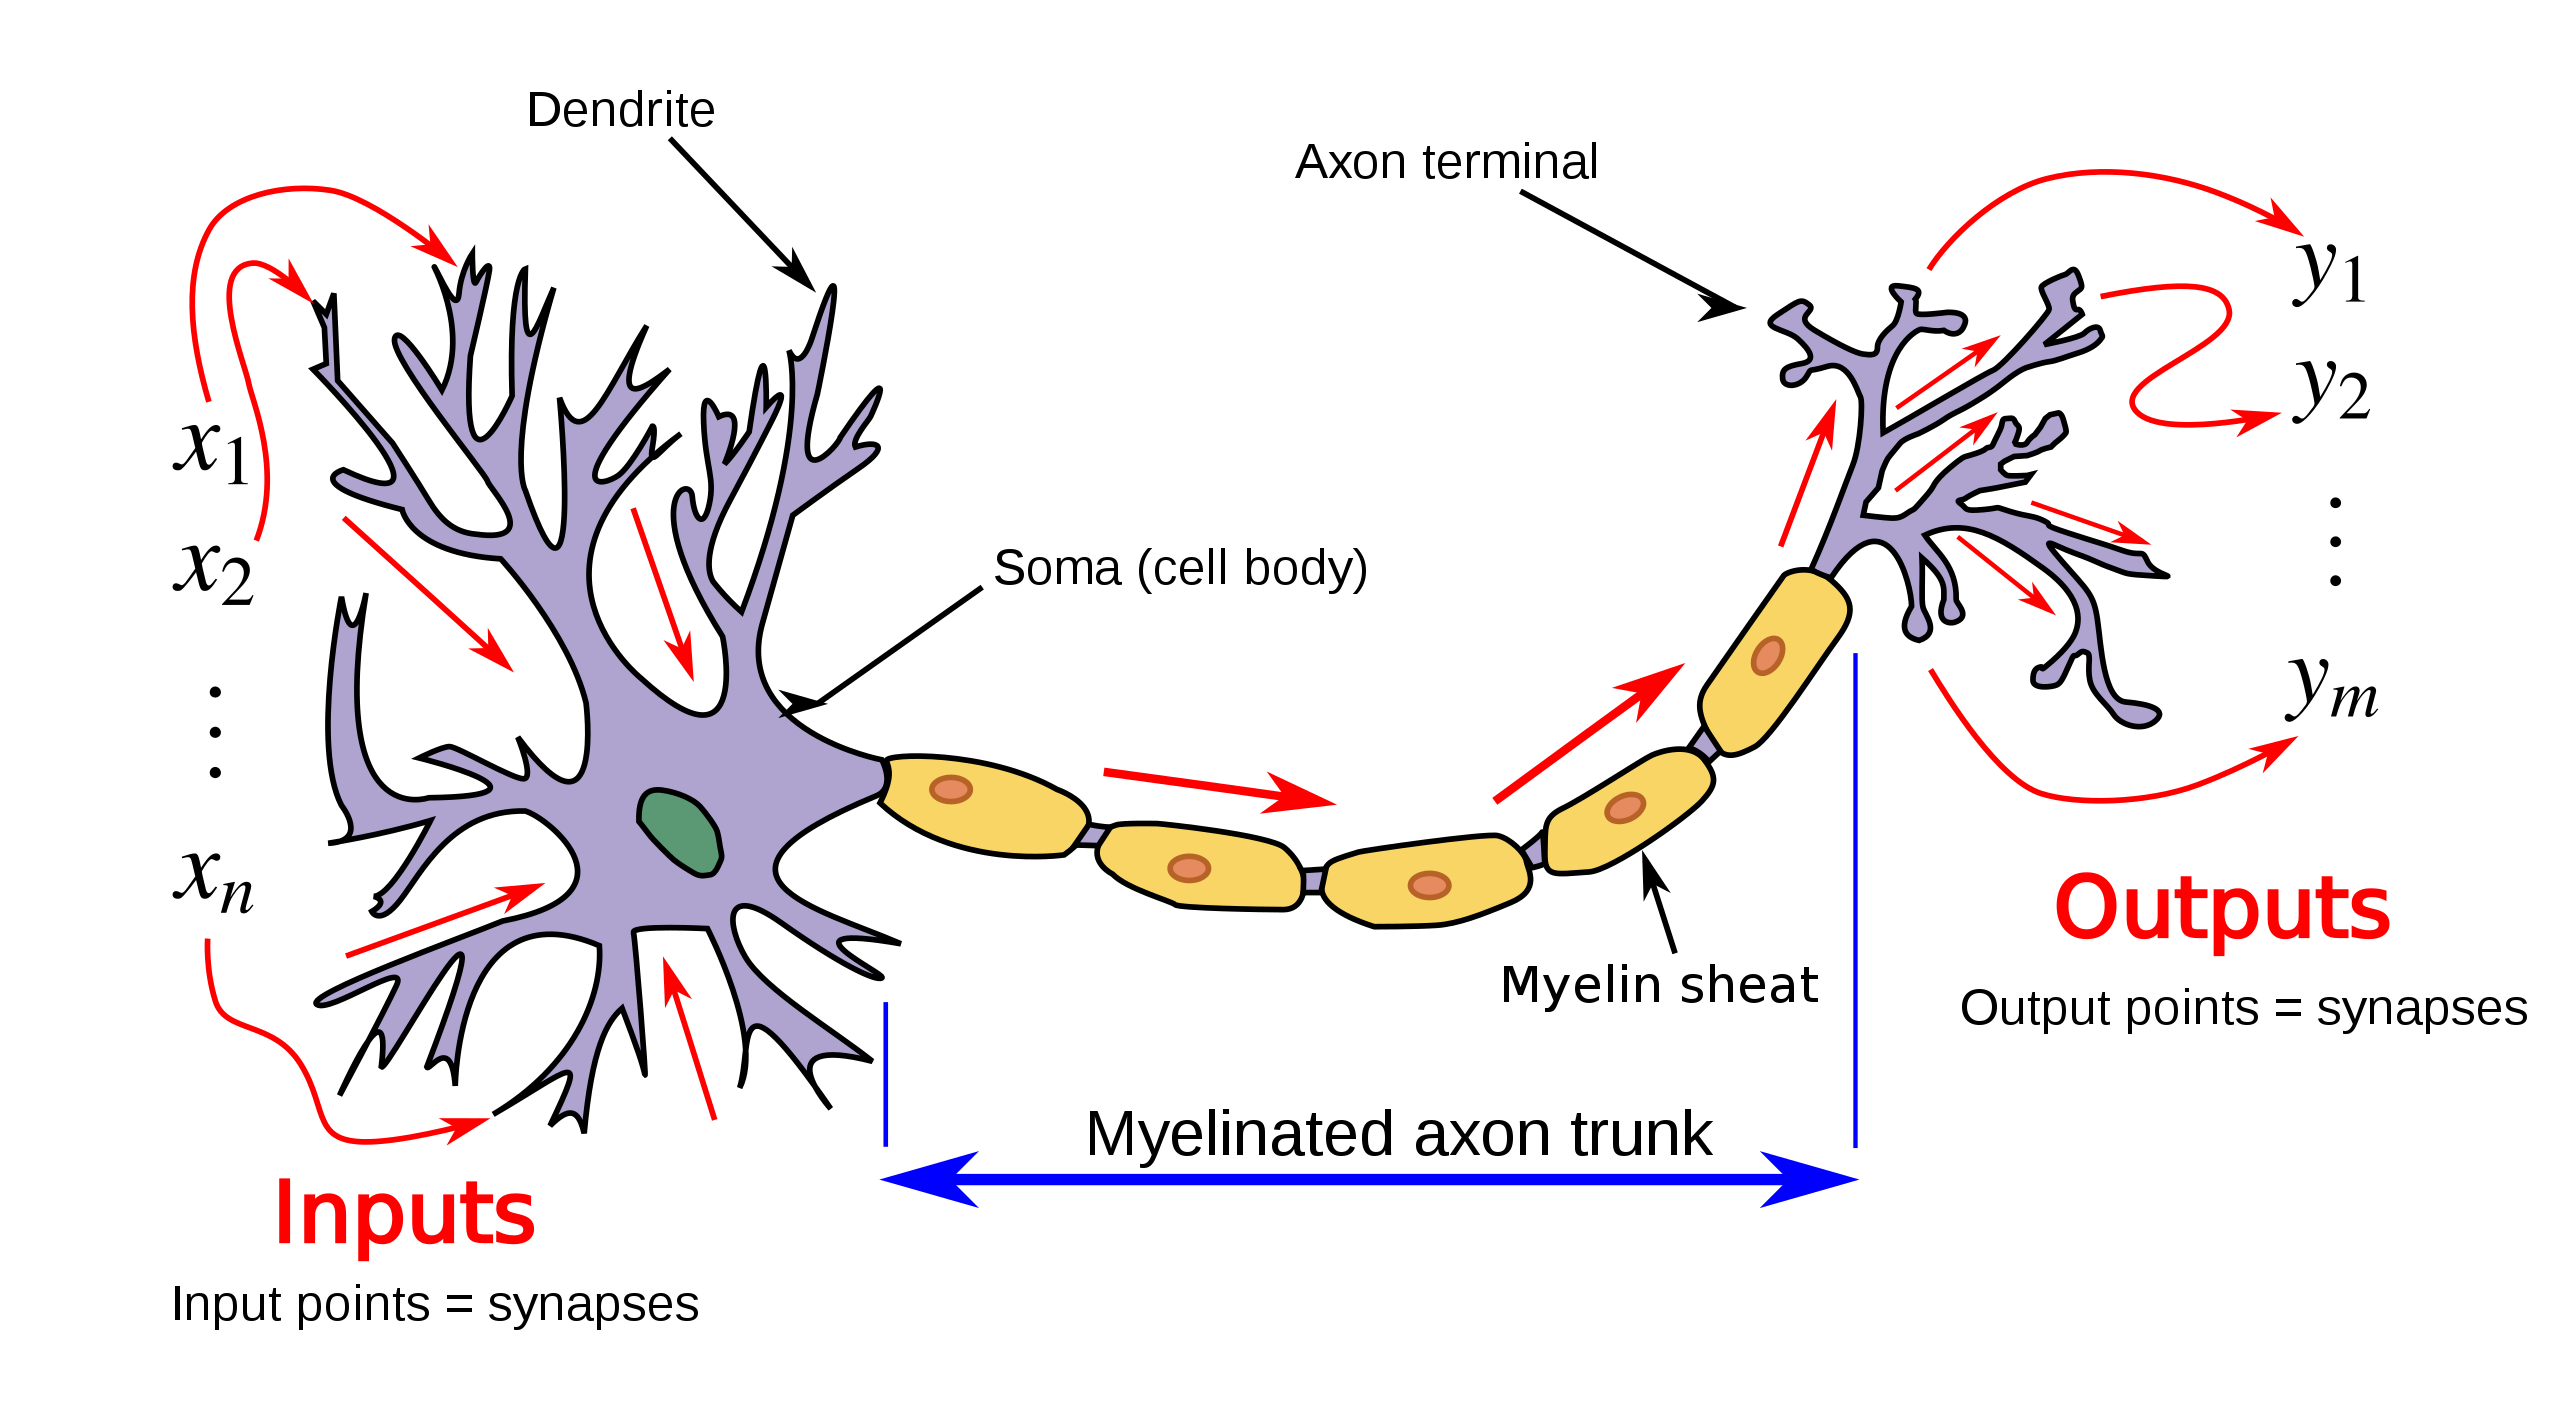
\includegraphics[width=0.9\textwidth]{neuron}

      \end{figure}
      \tiny{\href{https://en.wikipedia.org/wiki/Artificial_neuron\#/media/File:Neuron3.svg}{CC Prof. Loc Vu-Quoc}}
    \end{column}
    \begin{column}{0.48\textwidth}
      \begin{figure}
        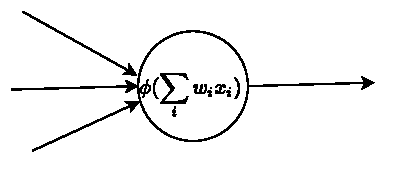
\includegraphics[width=0.9\textwidth]{neuron_02}
      \end{figure}
    \end{column}
  \end{columns}
  \note{
    \begin{itemize}
      \item The perceptron was invented in 1958 by Frank Rosenblatt      %
      \item It is a simplified model of a biological neuron.
    \end{itemize}
  }
\end{frame}


\begin{frame}{Can we learn these mappings? $\rightarrow$ Deep Neural Network}
  \begin{figure}
    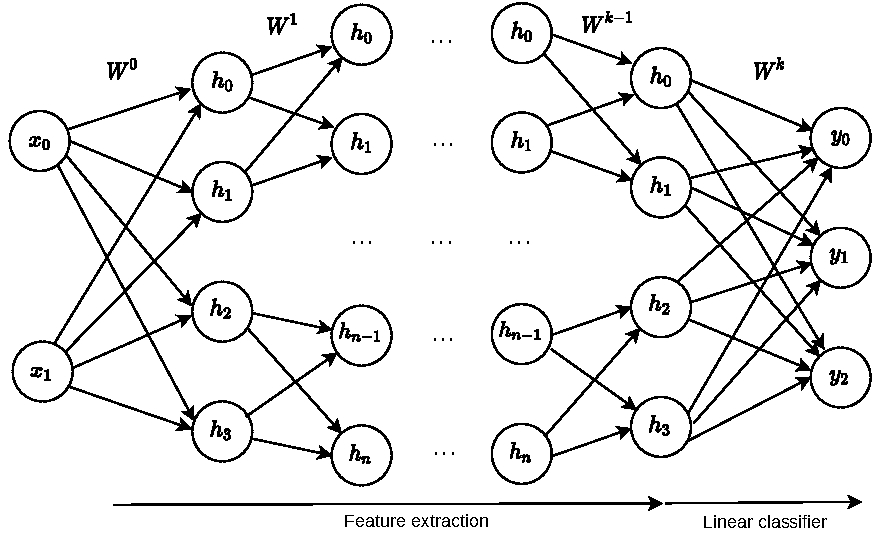
\includegraphics[width=0.6\textwidth]{neuron_03}
  \end{figure}
  \note{
    \begin{itemize}
      \item Adding more hidden layers to this, following the same principle, leads us to what is called deep learning.
    \end{itemize}
  }
\end{frame}


\begin{frame}{But wait. What's the derivative of this?}
  \begin{figure}
    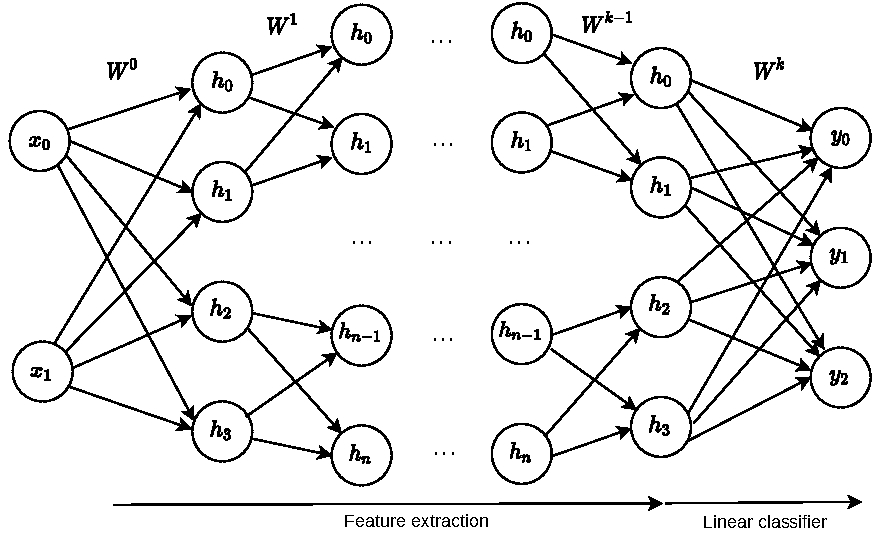
\includegraphics[width=0.6\textwidth]{neuron_03}
  \end{figure}
  \note{
    \begin{itemize}
      \item Manually deriving the derivative? Puhh ...
      \item Symbolic derivation leads to expression swell.
      \item Both are restricted to model definitions with closed-form expressions.
    \end{itemize}
  }
\end{frame}


\begin{frame}{But wait. What's the derivative of this?}
  \begin{equation*}
    \frac{\partial E(w)}{\partial w_{i}} \approx \frac{E(w+he_{i})-E(w)}{h}
  \end{equation*}
  \note{
    \begin{itemize}
      \item $e_{i}$ is the unit vector in the $i$th direction and $h$ is a small positive number.
      \item We could numerically evaluate the gradient for every weight.\\
      $\rightarrow$ Makes a full evaluation of the network for every weight necessary.
    \end{itemize}
  }
\end{frame}


\begin{frame}{But wait. What's the derivative of this? $\rightarrow$ Backpropagation}
    \begin{itemize}
      \item Fortunately, somebody figured, we could do this using the chain rule!
      \item The approach was developed many times but \\
            is widely used in Machine Learning mostly because of \\
            \textbf{Learning representations by back-propagating errors.} \\
            David E. Rumelhart, Geoffrey E. Hinton, and Ronald J. Williams; Nature; 1986
    \end{itemize}

  \note{
    \begin{itemize}
      \item
      \item
    \end{itemize}
  }
\end{frame}


\begin{frame}{Backpropagation}
  \begin{figure}
    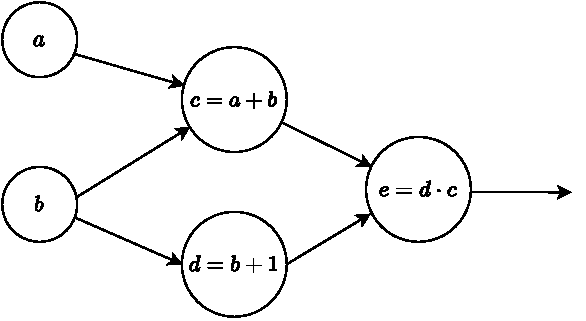
\includegraphics[width=0.6\textwidth]{backprop_00}
  \end{figure}
  \note{
    \begin{itemize}
      \item Let's look at the computational graph for the function $e = (a+b)(b+1)$
      \item Example from \url{https://colah.github.io/posts/2015-08-Backprop/}
    \end{itemize}
  }
\end{frame}


\begin{frame}{Backpropagation}
  \begin{figure}
    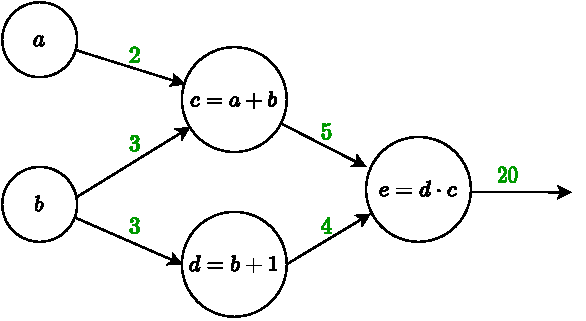
\includegraphics[width=0.6\textwidth]{backprop_01}
  \end{figure}
  \note{
    \begin{itemize}
      \item A forward pass through this graph for $a=2$ and $b=3$.
    \end{itemize}
  }
\end{frame}


\begin{frame}{Backpropagation}
  \begin{figure}
    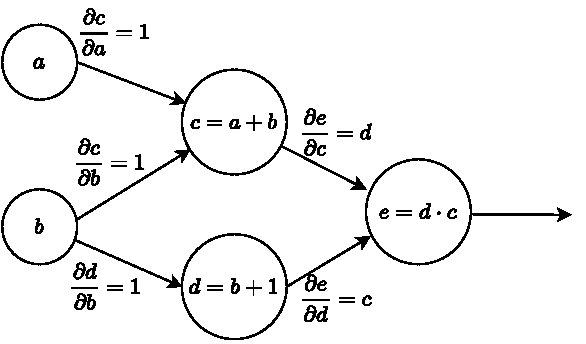
\includegraphics[width=0.6\textwidth]{backprop_02}
  \end{figure}
  \note{
    \begin{itemize}
      \item We can assign the partial derivative to each edge of the graph.
    \end{itemize}
  }
\end{frame}


\begin{frame}{Backpropagation}
  \begin{figure}
    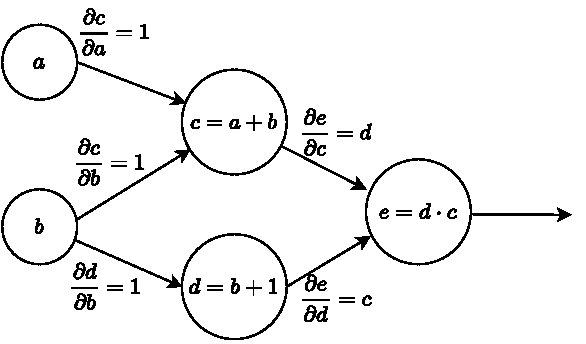
\includegraphics[width=0.35\textwidth]{backprop_02}
    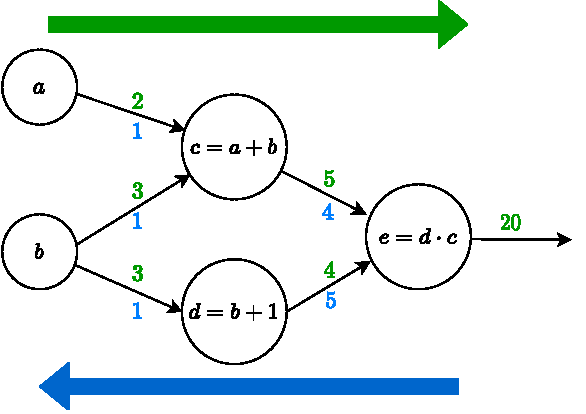
\includegraphics[width=0.6\textwidth]{backprop_03}
  \end{figure}
  \note{
    \begin{itemize}
      \item After a forward pass through the network, we can assign a value to all of the partial derivatives by doing what is called a backward pass.
    \end{itemize}
  }
\end{frame}


\begin{frame}{Backpropagation}
  \begin{columns}
    \begin{column}{0.75\textwidth}
      \begin{figure}
        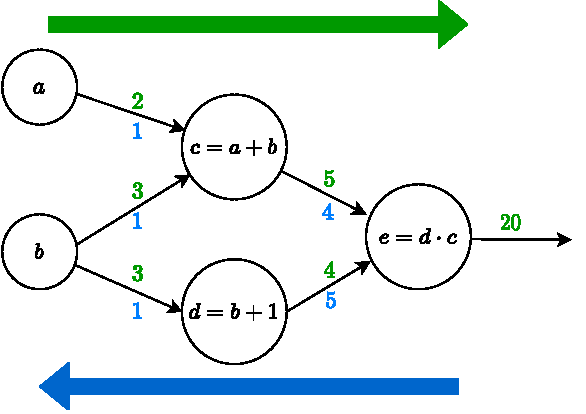
\includegraphics[width=0.9\textwidth]{backprop_03}
      \end{figure}
    \end{column}
    \begin{column}{0.2\textwidth}
      \begin{align*}
        \frac{\partial e}{\partial a} = 4\cdot 1 = \frac{\partial e(c(b))}{\partial c}\frac{\partial c(b)}{\partial b}
      \end{align*}
    \end{column}
  \end{columns}
\note{
    \begin{itemize}
      \item If we multiply the values of the partial derivatives of the nodes from output to parameter, we get the partial derivative of the full network with respect to this parameter.
      \item Which is nothing else than the application of the chain rule.
    \end{itemize}
  }
\end{frame}


\begin{frame}{Backpropagation}
  \begin{columns}
    \begin{column}{0.75\textwidth}
      \begin{figure}
        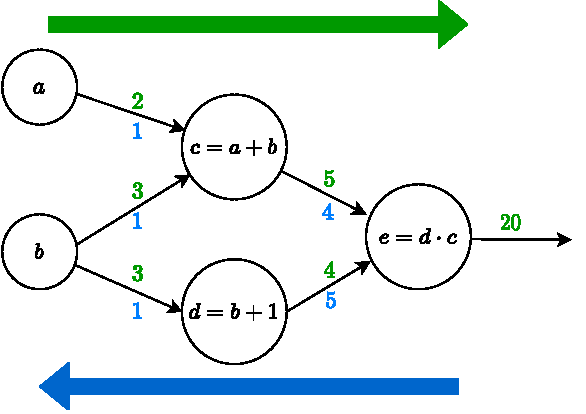
\includegraphics[width=0.9\textwidth]{backprop_03}
      \end{figure}
    \end{column}
    \begin{column}{0.2\textwidth}
      \begin{align*}
        & \frac{\partial e}{\partial b} = 4 \cdot 1 + 5 \cdot 1 \\
        & = \frac{\partial e(c(b))}{\partial c}\frac{\partial c(b)}{\partial b} + \frac{\partial e(d(b))}{\partial d}\frac{\partial d(b)}{\partial b}
      \end{align*}
    \end{column}
  \end{columns}
  \note{
    \begin{itemize}
      \item If there are multiple paths from output to parameter, we have to sum up all the derivatives at every node before propagating the further.
      \item This also corresponds to the chain rule in the multi variate case.
    \end{itemize}
  }
\end{frame}


\begin{frame}{Backpropagation}
  \begin{figure}
    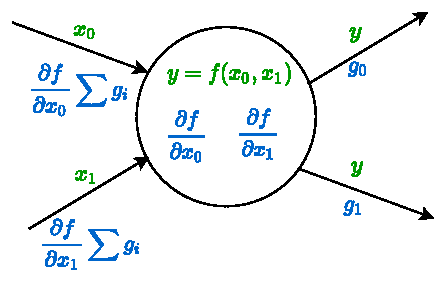
\includegraphics[width=0.6\textwidth]{backprop_04}
  \end{figure}
  \note{
    \begin{itemize}
      \item Every node needs to implement a function and the partial derivatives of that function with respect to its inputs. \\
            $\rightarrow$ The values of the partial derivatives of the network with respect to all parameters for a given input, can be computed with one forward and one backward pass.
    \end{itemize}
  }
\end{frame}


\begin{frame}{Backpropagation}
  \begin{figure}
    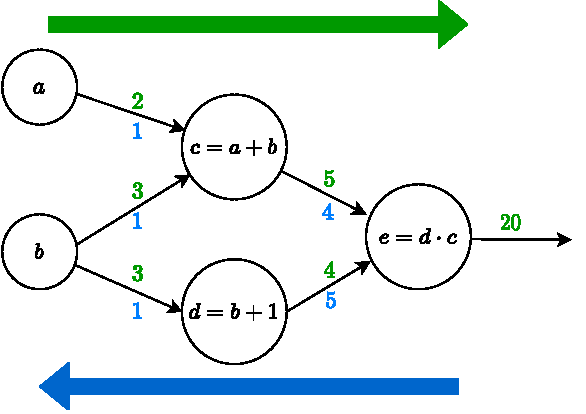
\includegraphics[width=0.6\textwidth]{backprop_03}
  \end{figure}
  \note{
    \begin{itemize}
      \item Activations (node output) of all layers have to be kept in memory for the backward path! \\
            $\rightarrow$ High memory consumption of the network during training. \\
            $\rightarrow$ (Yes, Backprop is dynamic programming.)
      \item Add-nodes distribute gradient equally.
      \item Multiply-nodes backpropagate their inputs as gradients.
      \item What does that mean e.g. for the $Wx$ operation? \\
            $\rightarrow$ Big input, big gradient on the weights! \\
            $\rightarrow$ Preprocessing of input data matters for gradient flow! \\
            $\rightarrow$ To understand and monitor gradient flow is crucial for successful training of neural networks. \\
    \end{itemize}
  }
\end{frame}


\begin{frame}{What about $\phi$?}

  \begin{columns}
    \begin{column}{0.48\textwidth}
      \begin{figure}
        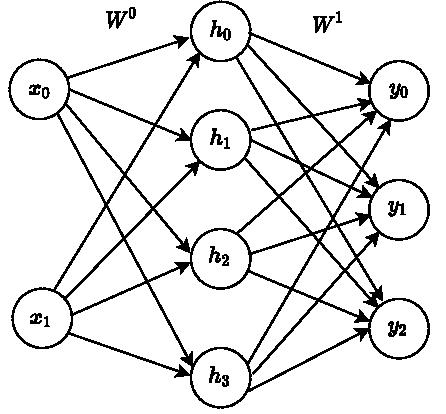
\includegraphics[width=0.9\textwidth]{neuron_01}
      \end{figure}
    \end{column}
    \begin{column}{0.48\textwidth}
      \begin{align*}
        y &= \sigma(W^{1}\phi(W^{0}x)) \\
        h &= \phi(W^{0}x)
      \end{align*}
    \end{column}
  \end{columns}

  \note{
    \begin{itemize}
      \item The vector $h$ is representation in learned feature space. \\
      $\rightarrow$ It can have any dimensionality.
      \item $\phi$ is called the activation function. \\
      $\rightarrow$ It needs to be non-linear. A purely linear mapping into a new feature space wouldn't help.
    \end{itemize}
  }
\end{frame}



\begin{frame}{Activation function}
  \begin{figure}
    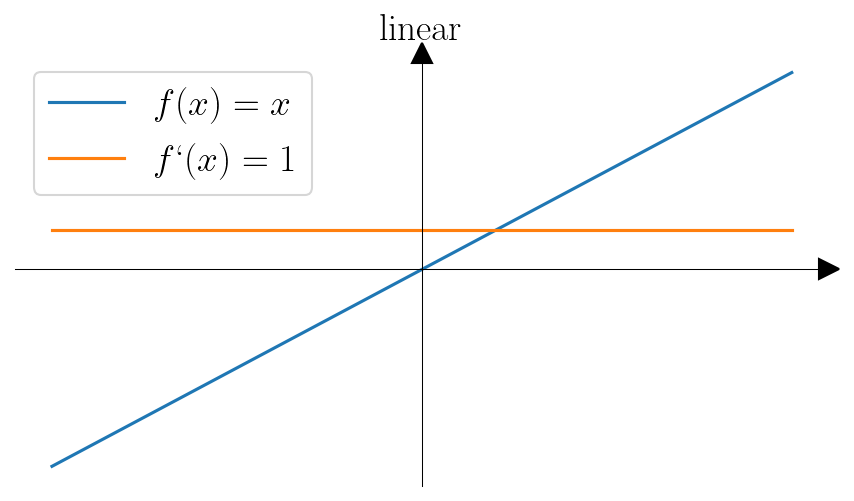
\includegraphics[width=0.33\textwidth]{activations_lin}\\
    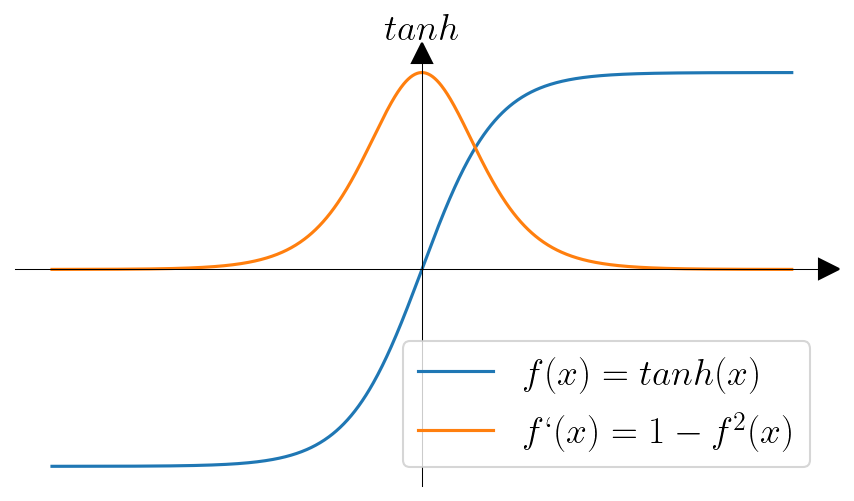
\includegraphics[width=0.33\textwidth]{activations_tanh}
    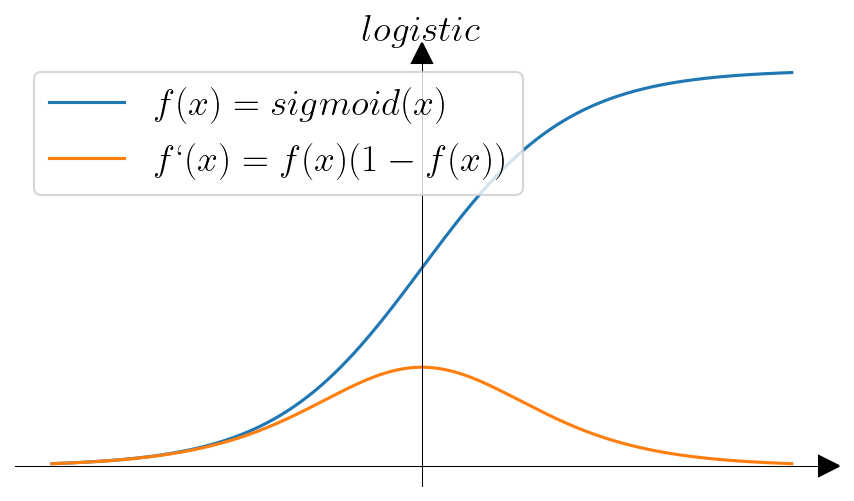
\includegraphics[width=0.33\textwidth]{activations_logistic}\\
    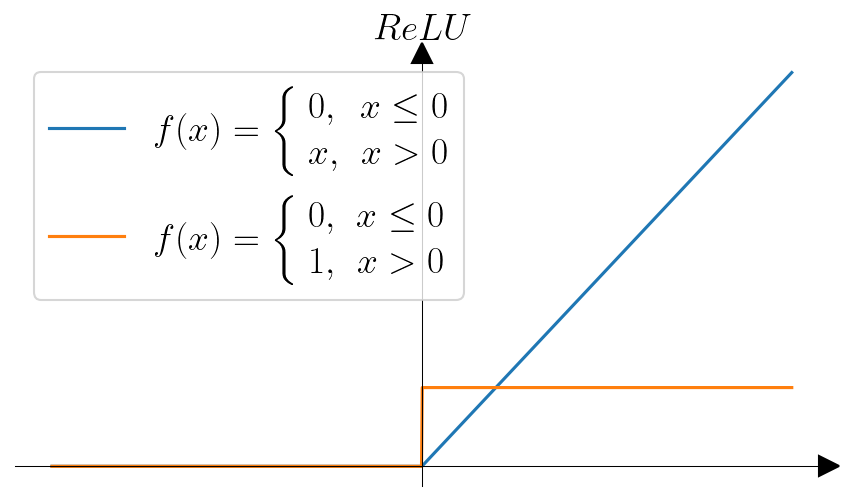
\includegraphics[width=0.33\textwidth]{activations_relu}
    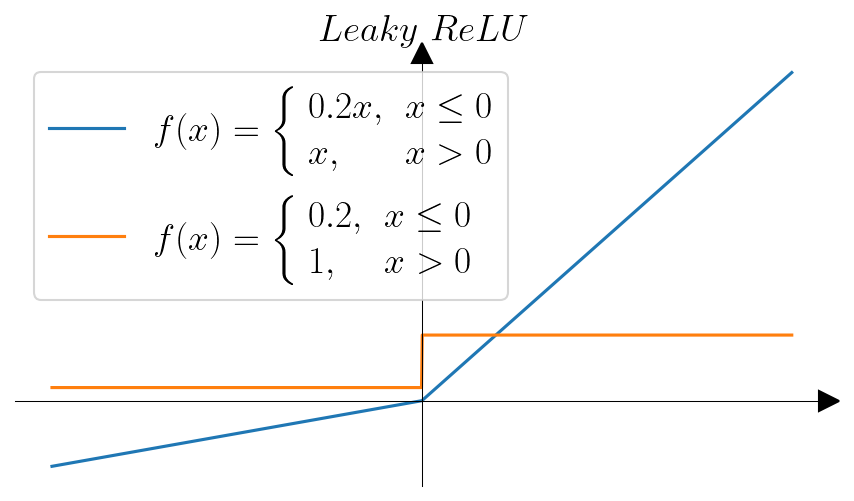
\includegraphics[width=0.33\textwidth]{activations_lrelu}
  \end{figure}

  \note{
    \begin{itemize}
      \item Let's have a look at possible activation functions.
    \end{itemize}
  }
\end{frame}


\begin{frame}{Overfitting}
  ``With great power comes great overfitting`` (Joseph Redmon)
  \vspace{1cm}
  \begin{figure}
    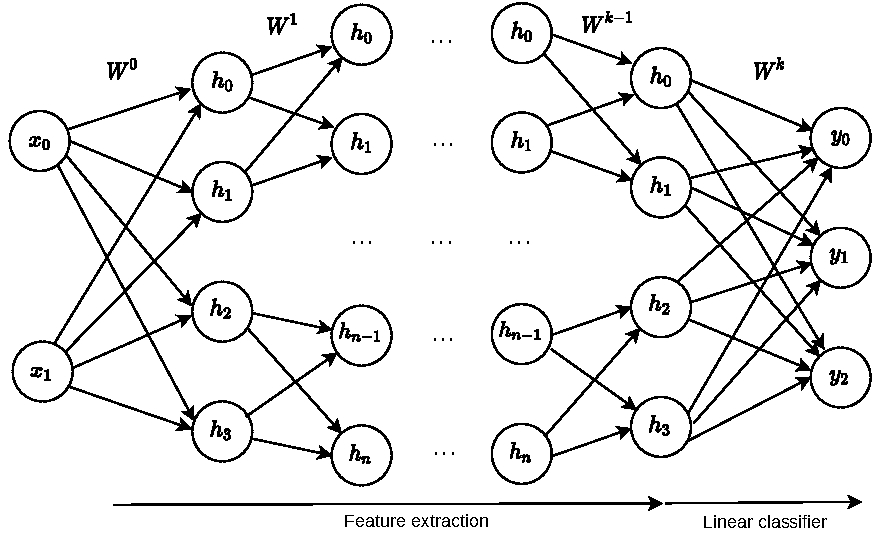
\includegraphics[width=0.6\textwidth]{neuron_03}
  \end{figure}
  \note{
    \begin{itemize}
      \item Deep neural networks have millions of parameters.
      \item They can learn to fit almost everything. But that's often not what you want.
    \end{itemize}
  }
\end{frame}


\begin{frame}{Bias and Variance in deep networks}
  \begin{figure}
    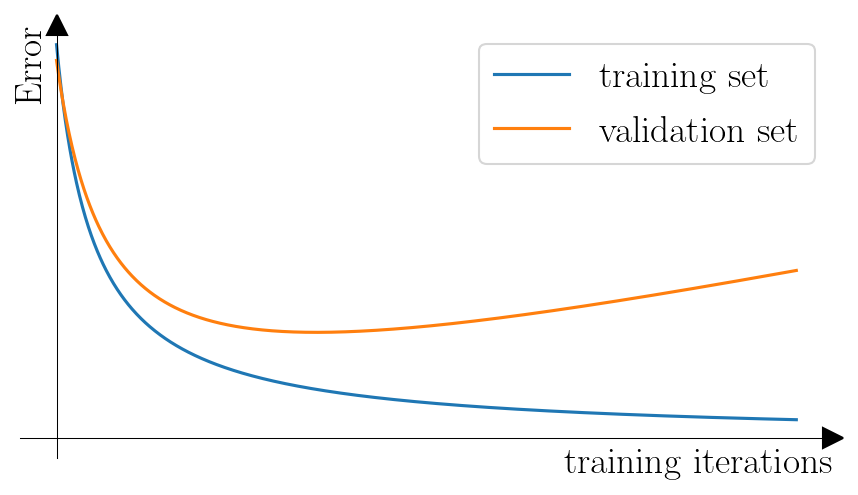
\includegraphics[width=0.8\textwidth]{training_curve}
  \end{figure}
  \note{
    \begin{itemize}
      \item When fitting a model with a gradient descent method, we should always look at the error on training and validation sets over training iteration.
      \item High bias \\
            $\rightarrow$ Increase model complexity
      \item High variance \\
            $\rightarrow$ More data and/or regularization
      \item In deep learning it's less of a trade-off between bias and variance. \\
            $\rightarrow$ We can increase model complexity accompanied with more data/regularization until bias is close to zero, without increasing variance much.
    \end{itemize}
  }
\end{frame}



\begin{frame}{Regularization}
    \begin{itemize}
      \item Early stopping
      \item Weight regularization
      \item Dropout
      \item Data augmentation
      \item Batch normalization
    \end{itemize}

  \note{
    \begin{itemize}
      \item Regularization is very important. Most approaches use multiple of the regularization methods listed here.
      \item We will discuss these methods in more detail in the exercises.
    \end{itemize}
  }
\end{frame}


\begin{frame}{A small MLP for computer vision}

  \begin{columns}
    \begin{column}{0.48\textwidth}
      \begin{figure}
        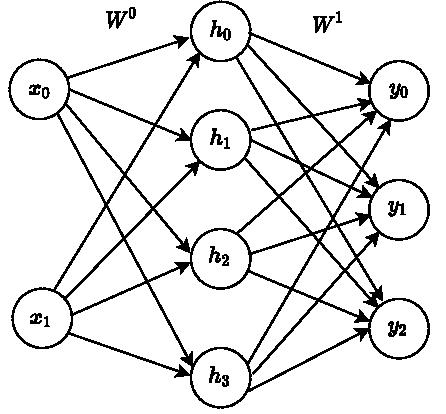
\includegraphics[width=0.9\textwidth]{neuron_01}
      \end{figure}
    \end{column}
    \begin{column}{0.48\textwidth}
      \begin{align*}
        128 \times 128 \times 3 & = 49152 \\
        16 \times 16 \times 36 & = 9216 \\
        \rightarrow 49152 \cdot 9216 + 9216 \cdot 10 & = 453076992 \approx 450 \cdot 10^{6}
      \end{align*}
    \end{column}
  \end{columns}

  \note{
    \begin{itemize}
      \item A small MLP with feature vector comparable to HOG.
      \item Input: an rgb image relatively low resolution\\
            $\rightarrow 128\times128\times3 = 49152 $
      \item Hidden layer: comparable to HOG with 36 dim feature vector computed from $8\times 8$ patches \\
            $\rightarrow$ $16\times16\times36 = 9216$
      \item Output neurons for e.g. 10 object classes \\
            $\rightarrow 49152 \cdot 9216 + 9216 \cdot 10 = 453076992 \approx 450 million$ parameters\\
    \end{itemize}

  }
\end{frame}
